\documentclass[runningheads,a4paper]{llncs}
%
\usepackage{natbib} % bibliography stuff
%
\usepackage{graphicx} % allows for working with images
\DeclareGraphicsExtensions{.pdf,.png,.jpeg} % configures latex to look for the following image extensions
%
\usepackage{setspace} % allows for configuring the linespacing in the document
%\singlespacing
\onehalfspacing
%\doublespacing
%
\usepackage{appendix}
%
\usepackage[toc]{glossaries}
\makeglossaries
%
\usepackage{amssymb}
\setcounter{tocdepth}{4}
%
\usepackage{url}
\urldef{\mailsa}\path|dkirwan@tssg.org, adavy@tssg.org|
\newcommand{\keywords}[1]{\par\addvspace\baselineskip
\noindent\keywordname\enspace\ignorespaces#1}

\begin{document}
\mainmatter  % start of an individual contribution

% first the title is needed
\title{Observing Jovian Decametric Radio Emissions\\
with a Software Defined Radio Telescope}

% a short form should be given in case it is too long for the running head
\titlerunning{Observing Jovian Decametric Radio Emissions}

% the name(s) of the author(s) follow(s) next
%
% NB: Chinese authors should write their first names(s) in front of
% their surnames. This ensures that the names appear correctly in
% the running heads and the author index.
%
\author{David Kirwan%
%\thanks{Please note that the LNCS Editorial assumes that all authors have used
%the western naming convention, with given names preceding surnames. This determines
%the structure of the names in the running heads and the author index.}%
\and Alan Davy\thanks{Supervisors} \and John Ronan\footnotemark[1]}
%
\authorrunning{D. Kirwan}
% (feature abused for this document to repeat the title also on left hand pages)

% the affiliations are given next; don't give your e-mail address
% unless you accept that it will be published
\institute{Waterford Institute of Technology,\\Dept of Maths and Physics,\\
Cork Rd, Waterford City, Ireland\\
\mailsa\\
\url{http://www.wit.ie}}

%
% NB: a more complex sample for affiliations and the mapping to the
% corresponding authors can be found in the file "llncs.dem"
% (search for the string "\mainmatter" where a contribution starts).
% "llncs.dem" accompanies the document class "llncs.cls".
%
\toctitle{Thesis Proposal}
\tocauthor{D. Kirwan}
\maketitle
%
%\begin{abstract}
%The abstract should summarize the contents of the paper and should
%contain at least 70 and at most 150 words. It should be written using %the
%\emph{abstract} environment.
%\keywords{radio astronomy, software defined radio, signal processing}
%\end{abstract}
%
\tableofcontents
%
\newpage
%
\section*{Introduction}
\addcontentsline{toc}{section}{Introduction}
%This is typically an outline description detailing the background	 to the problem.

\newglossaryentry{DAM}
{
  name={DAM},
  description={decameter radio emissions},
  sort=DAM
}
%
It was discovered in 1954 by \cite{burke55} that the planet Jupiter emits radio transmissions in the decameter (\gls{DAM}) range \textit{10-100 m wavelengths}, and the inner Jovian satellite Io appeared to have an effect on these emissions occurring \citep{belcher87}. Jupiter's radio emissions range between 4 MHz to 39.5 MHZ while emitting most strongly at 8 MHz or so \citep{wilkinson94}. However due to interference from human short wave radio sources between 4-15 MHz coupled with the attenuation of these signals or refraction off Earths ionosphere, the majority of emissions have been observed up in the 15-25 MHz range where this interference is less. The emission signal strength quickly diminishes above this range \citep{wilkinson94}.
%
\begin{figure}[here]
\centering
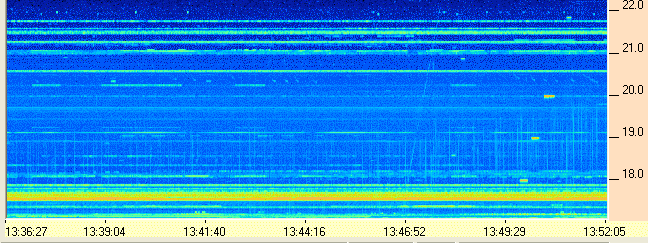
\includegraphics[width=8cm]{images/01}
\caption{Decametric Radio Emissions \citep{ashcraft13}}
\label{fig:dam_Emissions}
\end{figure}
%
Data collected by the two Voyager spacecraft in 1979 \citep{belcher87} and the later Galileo in 1995 \citep{kivelson96} added hugely to the understanding of the plasma interactions between Jupiter and Io and the source of the \gls{DAM} emissions. It was discovered that the Io has a thin atmosphere made up of a number of neutral gasses namely sodium, potassium, sulfur, and oxygen as shown in fig: \ref{fig:io_neutral_gasses}. It is generally thought these gasses have been emitted through volcanic activity on the surface of the moon \citep{belcher87}.
%
\begin{figure}[here]
\centering
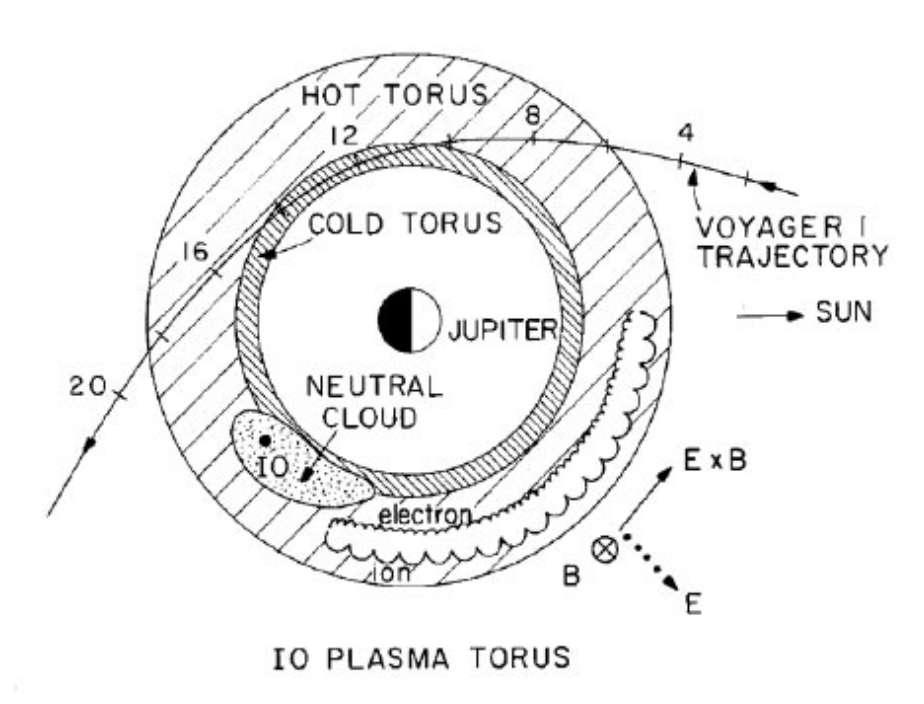
\includegraphics[width=8cm]{images/02}
\caption{Neutral Gasses in Orbit of Io \citep{belcher87}}
\label{fig:io_neutral_gasses}
\end{figure}
%
\newglossaryentry{IPT}
{
  name={IPT},
  description={Io Plasma Torus},
  sort=IPT
}
%
The gasses in orbit of Io have a very short life time, due to collisions with magnetospheric electrons. This gives rise to a plasma torus (\gls{IPT}) which corotates with Jupiter itself \citep{belcher87}. This can also be seen in fig: \ref{fig:io_neutral_gasses} which shows the \gls{IPT}. The local corotation speed of the plasma torus is faster than the Keplerian orbit of the moon, and the plasma overtakes Io in its orbit at \begin{math} 57 km\;s^{-1} \end{math} \citep{belcher87}.
%
\newglossaryentry{IFT}
{
  name={IFT},
  description={Io Flux Tube},
  sort=IFT
}
%
Fig \ref{fig:io_flux_tube} details a diagram of the Io Flux Tube (\gls{IFT}) which is a tube made up from Jovian of magnetic field lines \citep{belcher87} which thread the satellite. A large portion of the decametric emissions come from the area where the \gls{IFT} meets the Jovian ionosphere. 
%
\begin{figure}[here]
\centering
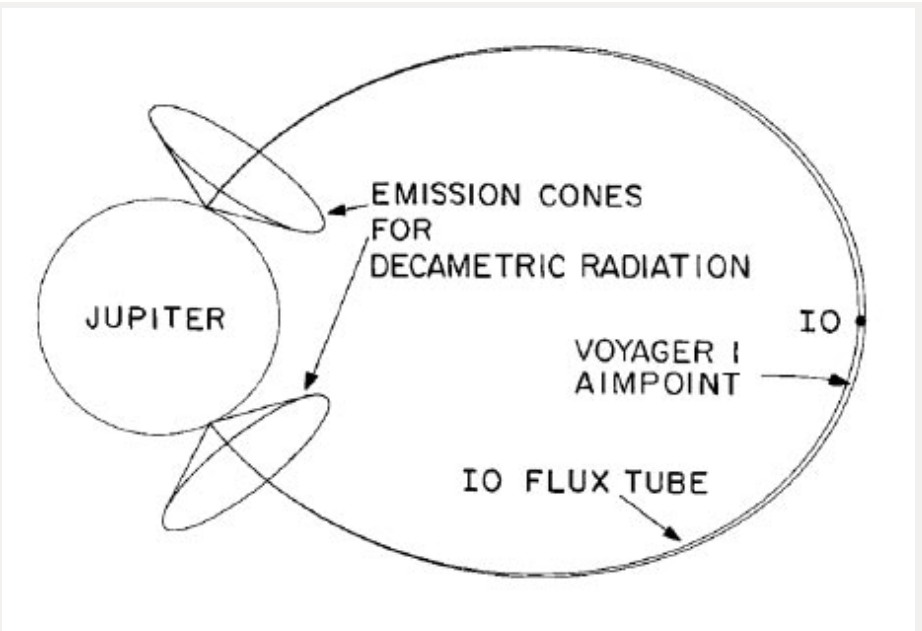
\includegraphics[width=8cm]{images/03}
\caption{Magnetic Flux Tube linking Jupiter and its satellite Io \citep{belcher87}}
\label{fig:io_flux_tube}
\end{figure}
%
As Io orbits within this flux torus it acts as a unipolar conductor \citep{bose08}, and Alfv\'en waves are regularly produced which carry an electric charge along the magnetic field lines between Jupiter and Io \citep{bose08}. These Alfv\'en waves reflect off Jupiters ionosphere at both north and south poles upto 9 times \citep{bose08} while following Io through its orbit, thereby acting as a standing wave. It appears the source of the \gls{DAM} emissions are largely due to these reflections of these Alfv\'en waves off Jupiter's ionosphere.
%%%%%%%%%%%%%%%%%%%%%%%%%%%%%%%%%%%%%%%%%%%%%%%%%%%%%%%%%%%%%%%%%%%%%%%%%%%%%%%%%%%%%%%%%%%
\newpage
\section*{Scope}
\addcontentsline{toc}{section}{Scope}
Students should identify whether the research outcomes are likely to have universal application or have a defined scope. This is important in gauging the extent to which the work is capable of independent replication.

Talk about the types of DAM emissions I'm interested in observing.

\begin{itemize}
  \item S-Bursts, short millisecond wideband bursts
  \item L-Bursts, long second wideband bursts
  \item N-Bursts, narrowband bursts
\end{itemize}
%
\citep{queinnec98}
%

Due to the latitude of Ireland being 53.3 degrees N, the telescope configuration will apply only to locations at this or a similar latitude, but will be universally applicable at this latitude without modification, and with relatively minor modifications can ensure the end solution can be used at all locations. \cite{kivelson96}

SDR Radio Telescope study Jupiter / Sun in the Decametric Band

\begin{itemize}
  \item Study Jupiter in the decametric band 3MHz - 40MHz
  \item Jupiter emissions near 20Mhz, are least likely to be interfered with from short wave transmissions
  \item Earths atmosphere is transparent at these frequencies during the night time
  \item Study Solar emissions during the day
  \item Solar emissions are strong enough to penetrate Earths atmosphere during the day
\end{itemize}


\begin{itemize}
  \item Low cost to deploy
  \item Can be run by an Amateur observer
  \item Mechanism for sending data from listening site back to a network connection (Ardtweeno)
  \item Backhaul system for capturing, processing and storage of listening site data
  \item API for accessing data, and or integrating into another system
  \item Amateur listening sites can compliment larger telescope arrays around the world
\end{itemize}


%
\newpage
%
\section*{Research Questions}
\addcontentsline{toc}{section}{Research Questions}
A clear, precise definition of the problem is very important to focus on the research activity. great care should be used in devising the research questions. They define the structure of the investigation/innovation that will be used and an essential metric of the quality of the dissertation is the degree to which the research question has/have been answered.

\begin{itemize}
  \item can I use this antenna to pick up signals from planetary bodies
  \item Signal Processing issues
  \item Can I address these natural signal noises
  \item Can I address these human signal noises
\end{itemize}

\subsection*{Potential Pitfalls}
\addcontentsline{toc}{subsection}{Potential Pitfalls}
Predecisions on how I want to collect data, creating the research questions itself I might need to carefully look at this, because I've made some initial ideas on how I want to collect this data.

Its going to be lower cost than other methods, or its using something new compared to other devices
 

\begin{itemize}
  \item Do amateur radio emissions adversely affect radio astronomy in the 15m band?
  \item What can be done using software defined radio to filter local radio interference from radio astronomy observations?
  \item How cheaply can a fully automated radio telescope listening station be built using current IOT technologies?
\end{itemize}

%
\newpage
%
\section*{Methodology}
\addcontentsline{toc}{section}{Methodology}
This should outline the approach and methodology being proposed by the student to address the research question.


%
\newpage
%
\section*{Preliminary Literature Review}
\addcontentsline{toc}{section}{Preliminary Literature Review}
This should contain a review of a number of books, journal articles and web references of relevance to the research area proposed. The literature should contain seminal and recent referenced research material that is categorised under a number of relevant sub-themes.

%WIP:

I've read about 15 papers already related to the background of the interactions between Jupiter and Io, and papers detailing results from similar telescopes to the design I intend to build. I've hit a paywall on some of the earliest seminal papers which were the first to detail the phenomenon of decametric emissions being emitted by the Jupiter-Io system. I will attempt to get a copy through the inter library loan system at WIT.


My literature review can be broken down into the following areas:

\begin{itemize}
  \item What are the decametric radio emissions and what are they caused by
  \item Research journals detailing potential radio telescope designs which could be replicated in order to collect DAM emissions
  \item I need to look into journals involving signal processing and maybe some rudimentary filtering or AI for identifying spurious signals
  \item Something else
  
\end{itemize}


%
\newpage
%
\section*{Contribution to Research Knowledge Anticipated}
\addcontentsline{toc}{section}{Contribution to Research Knowledge Anticipated}
%
A dissertation is a work of scholarly investigation that is grounded in the research literature and differs from a report or a book. It is judged on a prescribed set of academic criteria. Although the likely outcomes are tentative at hte start of the program, it is useful to incorporate them into the research proposal to help focus the work program.

%
\newpage
%
\section*{Description of the Experimental Design / Validation Methodology}
\addcontentsline{toc}{section}{Description of the Experimental Design / Validation Methodology}
%
A dissertation must employ rigorous scientific argument. The experimental design and the validation methodology must be specified in great detail in the proposal. At this proposal stage you should define clear evaluation criteria.


\begin{itemize}
  \item Identify data caused by lightning
  \item Identify data caused by human emissions
  \item Perform a site survey with the spectrum analyser
  \item Replicate the testbed at a second site
\end{itemize}


%
\newpage
%
\section*{Special Resources Required}
\addcontentsline{toc}{section}{Special Resources Required}
%
The research work may require access to specialised equipment, software, journals and so on.

Access to the HackRF or another similar SDR is required.
Access to the RadioJove Prediction software


%
\newpage
%
\section*{Main Milestones Anticipated}
\addcontentsline{toc}{section}{Main Milestones Anticipated}
%
Students should agree a number of milestones and their likely delivery dates with their supervisor at the start of the progress.


\begin{itemize}
  \item Design the testbed
  \item Build the telescope
  \item Perform a site survey with the spectrum analyser
  \item Replicate the testbed at a second site
\end{itemize}
%
\newpage
%
\bibliographystyle{plainnat}
\bibliography{bibliography/bibtex}
\addcontentsline{toc}{chapter}{Bibliography}
%
\newpage
%
\printglossaries
%
\newpage
%
\appendix
\section*{Appendix}
Here is some content in the appendix

\begin{subappendices}
\subsection*{How I became inspired}
Lorem ipsum dolor sit amet, consectetur adipiscing elit. Praesent ut egestas sapien. Sed vehicula, libero vitae ornare interdum, nunc felis rhoncus risus, ut lobortis quam ligula sed nunc. Suspendisse potenti. Proin lacinia ex dui, eu maximus justo consequat porttitor. Pellentesque sollicitudin rutrum ex hendrerit vestibulum. Etiam luctus leo vitae magna sagittis feugiat a vitae ligula. Maecenas suscipit interdum tincidunt. Etiam a sapien elit. Nam dictum sed felis non commodo.

%
\end{subappendices}

\end{document}


